\chapter{Simulation: file EC.vtu}
\section{Analysis of the energy levels}
After importing the file \texttt{DQD-EC.vtu} through the Paraview software,
we can analyze the energy values of the bottom of the conduction band in the different regions of the device.
For our porpuses, we first perform a "slice" of the 3D structure along the plane $z=-2.5$nm: we choose to do it at this 
height because, from the definition of the geometry described in the previous chapter, this is the height where the channel is located between the source and drain condacts. 
In particular, the Silicon layer where the quantum dots are formed extends from $z=0$nm to $z=-10$nm, so the plane at $z=-2.5$nm is well within the channel and allows us to analyze the energy levels in the region of interest.

\begin{figure}[h]
\center
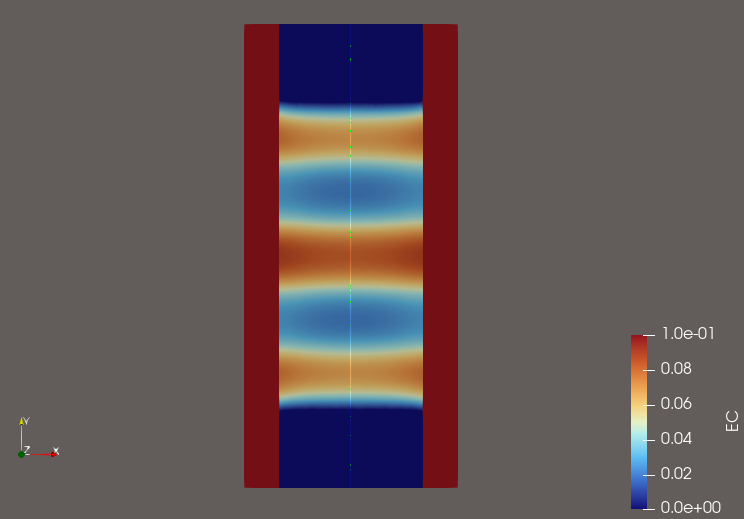
\includegraphics[width=1\textwidth]{leo_part/ec_topview.png}
\caption{Top view of the conduction band energy levels within the channel, the colorbar is in eV.}
\label{ec_topview}
\end{figure}

As we can see in the figure \ref{ec_topview}, the energy levels follow 

